%!TEX root = ../../prace.tex


\section{Elektrická síť}
\label{sec:energyNet}

Spojování bloků do elektrické sítě nevyžaduje žádnou speciální logiku. V~rámci přidávání bloku do herního světa budeme potřebovat vědět o~sousedních blocích (TODO stromy). Pokud bude vazba se sousedním blokem vyhodnocena jako validní vodivý spoj, může se nově připojený blok připojit ke stávající síti, v~níž je i~daný sousední blok.

Pokud budeme vycházet z~premisy, že každý blok je zapojen právě v~jedné elektrické síti a~všechny bloky v~rámci jedné elektrické sítě jsou mezi sebou vodivě spojeny, tak nutně musíme dojít k~závěru, že při manipulaci s~blokem budeme muset elektrické sítě aktualizovat. Přidáním bloku jsme bychom mohli vodivě propojit dvě či více sítí, při odebírání se nám daná elektrická síť může rozpadnout na více samostatných komponent. Těchto elektrických sítí může vznikat a~zanikat velké množství. Stačí si uvědomit, že k~bloku \nameref{blocks:A1} o~maximální možné velikosti můžeme připojit až 600 bloků, které budou patřit do stejné sítě (pro každou stěnu máme 100 bloků stejného typu a~minimální velikosti, uspořádaných do šachovnicového vzoru). Pokud pak odebereme centrální blok, může nám vzniknout právě až 600 nových elektrických sítí. Navíc, díky počasí se může stát, že bloky budou odebírány ze světa zcela neuspořádaně (na základě náhodně udělovaného poškození). Musíme tedy vymyslet algoritmus, jak pro všechny bloky v~herním světě udržovat správné informace o~jejich síti.

Protože nemůžeme nic předpokládat o~tom, jak se budou bloky v~elektrické síti chovat, musíme při změně (přidání či odebrání) nějakého bloku v~síti provést přepočítání. Nejjednodušší bude varianta na \textit{algoritmus vlny}. Jednotlivé sítě budeme podle potřeby odstraňovat či slévat. Popišme si nyní pravidla, která budeme muset ve hře mít. Jako sousedy budeme chápat bloky dostupné skrze vodivé spojení.

\subsubsection{Přidávání bloku}
Platí, že každý blok přidaný do herního světa si vytvoří svoji vlastní elektrickou síť.
(TODO kontrola enums níže)
\begin{enumerate}
	\item Pokud blok nemá žádné sousedy, nemusí dělat nic (svoji síť už má)
	\item Pokud mají všichni sousedé stejnou síť, blok se k~ní připojí
	\item Pokud mezi sousedy existují alespoň dvě různé elektrické sítě, blok si vytvoří novou elektrickou síť, propojí ji s~ostatními sítěmi a~vyvolá přepočet sítí
\end{enumerate}

\subsubsection{Odebírání bloku}
Platí, že každý odebíraný blok z~herního světa vždy odstraní síť, ve které je připojen, a~pro všechny jeho sousedy jsou vytvořeny nové sítě.

\begin{enumerate}
	\item Pokud blok nemá žádné sousedy, svoji síť ze hry odstraní a~dále nedělá nic
	\item Pokud má blok právě jednoho souseda, odpojí od se od dané sítě
	\item Pokud má alespoň dva sousedy, pro každého vytvoří novou síť a~vyvolá přepočet sítí
\end{enumerate}

\subsection{Udržování konzistence elektrických sítí}

Jak je vidět z~předchozí kapitoly, objektů k~aktualizaci může být velmi mnoho. Nesmíme však dopustit, aby se nám při přepočítávání začala hra zpomalovat či přímo zasekávat\footnote{Tato situace může snadno nastat, protože herní a~renderovací smyčky se na konci svých cyklů synchronizují, aby pro výpočet dalšího framu začínaly stejně.}. Opět máme více možností řešení, jak se k~tomuto problému postavit. 

Jedním z~možných řešení je spuštění výpočtů na samostatném výpočetním vlákně. Zde bohužel narážíme na problém, že výpočty ve vláknech v~\UEu{} nemohou přímo přistupovat k~herním objektům a~tudíž je nutné používat pomocných datových struktur a~výsledky poté zpětně propagovat. Kromě toho také narážíme na problém, kdy v~případě velmi silné bouře kyselých dešťů bude nejspíše často nutné výpočet předčasně ukončit a~spustit znovu.

My navrhujeme následující algoritmus, využívající front požadavků ke zpracování a~omezení výpočetního času. Ještě musíme zmínit, že také využívá toho, že jak elektrická síť, tak každý blok v~ní si nese informaci o~stavu. Ty jsou tři:
\begin{itemize}
	\item Nevalidní
	\item Ve výpočtu
	\item Validní
\end{itemize}
Volba stavů je zřejmá a~vychází z~principů algoritmu vlny. Dalším netriviálním faktem je, že v~algoritmu existuje fronta sítí k~přepočítání, přičemž každá taková má svoji frontu bloků v~síti k~přepočítání. Hlavním krokem algoritmu je pak výběr sítě k~přepočítání a~provedení jednoho kroku přepočtu. Následně, pokud má tato síť stále nějaké bloky k~přepočtu, je zařazena na konec přepočítávací fronty a~tam čeká, dokud nebude opět vyzvednuta. Může se však stát, že jistou posloupností kroků při mazání bude tato síť označena jako nevalidní a~dále se přepočítávat nebude.

Algoritmus bude mít přidělené nějaké maximální kvantum času, řekněme tak, aby při jeho výpočtech hra dosahovala alespoň 30 snímků za sekundu. Tím vcelku jednoduchým a~elegantním způsobem zajistíme přepočty i~pro velice rozsáhlé sítě. Samozřejmě je nutné, aby hra počítala s~tím, že elektrická síť a~bloky v~ní mohou být ve stavu \textit{ve výpočtu} a~tomu přizpůsobovat další funkcionalitu (například nevyužívat zdrojů takovéto sítě, dokud blok není \textit{validní} -- pak je možné využívat pouze dalších validních bloků, tedy těch, které již byly zpracovány algoritmem).

TODO tabulka případů, říct, že tohle bude komponenta



\section{Bloky v~herním světě}
\label{sec:blocksWorld}

Způsobů, jak reprezentovat bloky ve světě, je více, takže bychom měli jednotlivé varianty porovnat a~vyhodnotit. V~této chvíli si také musíme určit, jak velký chceme náš herní svět mít. Na základě tohoto důležitého požadavku budeme posuzovat vhodnost jednotlivých implementací. My jsme se rozhodli, že hráči nabídneme rozsáhlý svět čtvercového půdorysu o~rozloze $100\,\ km^2$ a~výšky $5\,\ km$. Teď trochu předběhneme a~prozradíme, že nás k~tomuto rozhodnutí vedla snaha, aby datové struktury nebyly úplně triviální (třeba dvourozměrné pole). Zároveň s~tím si ale uvědomujeme, že správně by hra měla řešit takto velký svět tak, aby i~velké množství bloků hru nezpomalovalo či dokonce neshodilo celou hru (třeba z~nedostatku paměti RAM). Nicméně jak jsme zmínili v~kapitole (TODO ref), budeme v~této práci očekávat takové množství bloků, jejichž počet hra bez problémů zvládne.

Námi definované hranice herního světa se u~bloků projeví tak, že v~rámci herního světa můžeme mít až  $50~000 * 50~000 * 25~000$ bloků jednotkové velikosti, což je opravdu mnoho. Prvně se tedy zaměříme na to, jak vůbec můžeme bloky reprezentovat a~zároveň s~tím budeme řešit, jak se vypořádat s~různými rozměry bloků.

\subsection{Použití dvourozměrného pole}

Představme si, že bychom herní svět reprezentovali polem. Pak bychom potřebovali 62~500~\textit{miliard} ukazatelů, z~nichž by naprostá většina byla prázdných (\textit{NULL}ových). Pro jednoduchost počítejme, že jeden ukazatel má velikost 4B a~že 1 kB je roven 1000 B. Pak dostáváme, že bychom potřebovali alokovat 250 TB dat. Možná, že za několik let to nebude problém, ale v~současné době nám to tak trochu vadí, takže se zkusme zaměřit na efektivnější datové struktury.

\subsection{Stromové struktury}
\label{subsec:trees}

Jako rozumný nápad se jeví použití stromových struktur, které nám budou reprezentovat svět podle skutečně zabraných pozic v~herním světě. Kdybychom povolili volnou počáteční rotaci, zřejmě bychom museli přistoupit k~nějaké variantě \textit{clusterů}, tedy shluků bloků ve stejné ortogonální mřížce. Protože tuto vlastnost nepovolujeme, můžeme se zabývat jinými datovými strukturami, například:

\begin{itemize}
	\item Použití Octree
	\item Použití některé varianty AABB stromů
\end{itemize}

Pojďme si tedy tyto možnosti rozebrat.

\subsubsection{Octree}
Octree je stromová datová struktura, ve které vrchol reprezentuje nějaký objem a~jeho 8 potomků tento objem rovnoměrně dělí na menší části. Obvykle vrcholy této struktury reprezentují krychle v~nějakém prostoru. Pokud se zamyslíme, jak by náš svět byl v~této struktuře reprezentován, dojdeme k~tomu, že kořenový vrchol této struktury by měl 4 potomky vždy prázdné. Ačkoliv to není nijak zásadní nevýhoda, podívejme se na alternativní řešení.

\subsubsection{K-D tree}
K-D strom je datová struktura, která je velmi podobná Octree, ale na rozdíl od ní má pouze 2 potomky. Vrchol, který se nachází v~nějaké hladině, totiž svůj objem rozdělí do dvou polovin v~závislosti na dané hladině. Takto je možné reprezentovat vícedimenziální prostory, kdy jednotlivé hladiny reprezentují dělení pro jednotlivé souřadnice. Každá následující hladina této struktury pak představuje dělení podle následující souřadnice v~daném prostoru. Pro n-dimenzionální prostor pak (n+1) hladina (počítáno od jedné) opět dělí prostor podle první souřadnice.

Tato datová struktura se nám zamlouvá více, protože při správné implementaci můžeme \uv{beztrestně} změnit rozměry herního světa (pokud to bude potřeba) a~nebudeme muset měnit implementaci reprezentace bloků v~herním světě. Navíc budeme chtít, aby byla hloubka stromu co nejmenší, takže navrhujeme optimalizaci, kdy blok ve stromě může být v~daném vrcholu uložen jako \uv{jedináček}. (TODO více níže)

\subsection{Reprezentace bloku}

Abychom si usnadnili indexování bloků, budeme uvažovat, že bloky jsou indexovány v~rozsahu [-25~000, 25~000] ve všech souřadnicích a~jednotkový blok na herních souřadnicích [0, 0, 0] bude v~\UEu{} reprezentován na pozici [0, 0, 0]. Z~toho nám vyplývá, že můžeme snadno \UEu{} říci, kam má daný blok umístit -- stačí nám naše herní souřadnice vynásobit konstantou velikosti hrany základního bloku. Dále budeme uvažovat, že v~ose Z~(tedy vertikální ose) budeme mít bloky na pozicích v~intervalu [0, 25~000]. Z~toho nám vyplývá, že rovina, která bude reprezentovat povrch planety, bude mít Z-kovou souřadnici rovnu $-10$ a~všechny bloky budou umístěny nad ní.

Vyřešili jsme, jak přistupovat k~jednotkovým blokům, ale ještě musíme vyřešit případ škálovaného bloku. Využijeme toho, že \UE{} nám nabízí škálování herních objektů. Protože následující text je koncepčně velmi složitý, prozradíme pravidla fakta pro krychli o~rozměrech [2, 2, 2] v~bodech.

\begin{itemize}
	\item Vizuální reprezentace krychle je centrovaná, takže pokud ji umístíme na souřadnice [0, 0, 0] v~souřadnicovém systému \UEu{}, fyzické hranice bloku budou $\{ [-20, 20], [-20, 20], [-20, 20]\}$ v~osách $\{X, Y, Z\}$.
	\item Z~toho důvodu, že máme povrch planety umístěn v~ose $Z = -10$, nejbližší validní umístění tohoto bloku je na pozici [0, 0, 10] v~souřadnicovém systému \UEu{}.
	\item Blok bude mít naši herní souřadnici podle umístění svého středu. Pokud střed neodpovídá přesné pozici jednotkového bloku v~herním světě, \textit{virtuálně} se posouvá na nejbližší nižší pozici ve všech osách po se zarovnáním do herní mřížky. Takže herní souřadnice našeho bloku zůstanou [0, 0, 0]. 
	\item Pokud bychom měli výšku krychle 3, herní souřadnice by pak byla [0, 0, 1] (střed bloku odpovídá konkrétní pozici jednotkové krychle v~rámci herního světa) a~blok by byl na pozici [0, 0, 20] v~souřadnicovém systému \UEu{}.
	\item Rotace bloku jsou vůči chápanému středu bloku v~rámci našeho souřadnicového systému. Z~toho vyplývá, že námi uvažovaná krychle bude při rotaci kolem vertikální osy měnit i~svoji pozici v~rámci souřadnicového systému \UEu{}.
\end{itemize}

Z výše uvedených faktů je vidět, že ve hře budou muset existovat pravidla pro výpočty mezi souřadnicovým systémem naší hry a~souřadnicovým systémem \UEu{}. Dále z~toho vyplývá, že pokud má blok netriviální škálování, dle výše uvedených pravidel může inherentně \uv{zabrat} některé pozice v~našem souřadnicovém systému a~jiné bloky pak tento prostor nemohou obývat. To je skvělý výsledek, protože tím máme vyřešené konkrétní pozice a~nemohou nám nastat konflikty umístění bloků.

Další výhodou, kterou nám tato pravidla přináší, je snadný výpočet hranic bloku. Toho můžeme úspěšně využít při práci s~naším K-D tree, kdy si pro dva bloky z~jejich umístění v~našem souřadnicovém systému, velikosti a~rotace můžeme spočítat hranice bloku, třeba jako Min-Max box\footnote{Jako Min-Max box budeme chápat strukturu, která je popsána dvěma vektory, které představují minimální a~maximální hranice. Ve 2D prostředí by to byl obdélník s~udáním levého dolního rohu a~pravého horního rohu.}. Jednoduchým a~rychlým výpočtem pak můžeme analyzovat, jestli mají nějaký netriviální průnik, jestli se dotýkají apod.

Abychom to celé uzavřeli, tak budeme chtít, aby jednotlivé vrcholy našeho K-D stromu znaly svoji reprezentaci v~podobě Min-Max boxu. Tím získáme výhodu rychlého vyhodnocení, zda je možné umístit nový blok na souřadnice udané hráčem. Dále, budeme chtít, aby bloky měly vazbu na náš K-D strom. Cílem je dosáhnout toho, aby blok mohl vyhledávat své sousedy \uv{odspodu} a~hledání tak bylo velmi rychlé.


\subsection{Zapojení do rozpoznávání tvarů}

Vzhledem k~dynamicky škálovatelným bloků budeme požadovat, aby bylo možné bloky skládat do tvarů libovolným splňujícím způsobem. Dobře je to vidět na následujícím obrázku \ref{fig:konfig}:

\begin{figure}[!ht]\centering
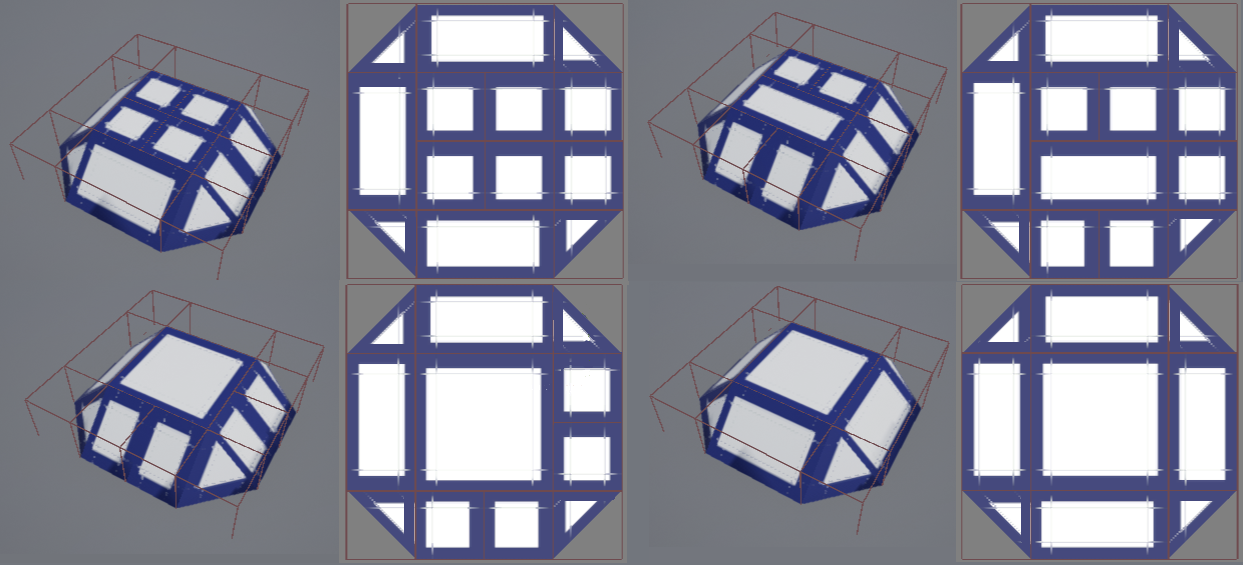
\includegraphics[ width=140mm]{../img/analysis/konfigurace}

\caption{Ekvivalentní konfigurace tvaru. Zdroj: StackOverflow.com~\citep{so_pattern}}
\label{fig:konfig}

\end{figure}

\FloatBarrier

Všechny tvary z~obrázku \ref{fig:konfig} by měly dohromady tvořit stejný tvar, ačkoliv splnění tohoto tvaru bylo u~každého tvaru rozdílné. Tento přístup však přináší mnoho problémů. Pro příklad uvažme rozklad bloku \nameref{blocks:A5} netriviální velikosti (kupříkladu [2,~1,~2], tedy šířky jednotkového bloku). Je zřejmé, že stejného tvaru je možné dosáhnout použitím dvou stejných bloků velikosti [1,~1,~1] a~jednoho bloku \nameref{blocks:A2} velikosti [1,~1,~1] (pokud budeme uvažovat, že tyto dva bloky je možné vzájemně kombinovat).

Z předchozích poznatků vyplývá, že definice nějakého komplexního tvaru, složeného z~různých typů bloků
(TODO dokončit)


